% generated by scripts/pkl_to_latex.py
% source PKL : vscan_v1_L6_Ne6_U10_t1_mode-uniform_nmin2_solver-gcg_full_restarts10_iter300_kmax5_tol1em09_V0to12_N25-ebabade1a2a1.pkl
% scan type  : vscan
% state      : gs
% quantity   : purity
% requires   : \usepackage{pgfplots} \pgfplotsset{compat=1.18}
% colours match the matplotlib PDF (tab10 cycle)
\definecolor{gmeC0}{HTML}{1F77B4}
\definecolor{gmeC1}{HTML}{FF7F0E}
\definecolor{gmeC2}{HTML}{2CA02C}
\definecolor{gmeC3}{HTML}{D62728}
\definecolor{gmeC4}{HTML}{9467BD}
\definecolor{gmeC5}{HTML}{8C564B}
\definecolor{gmeC6}{HTML}{E377C2}
\definecolor{gmeC7}{HTML}{17BECF}

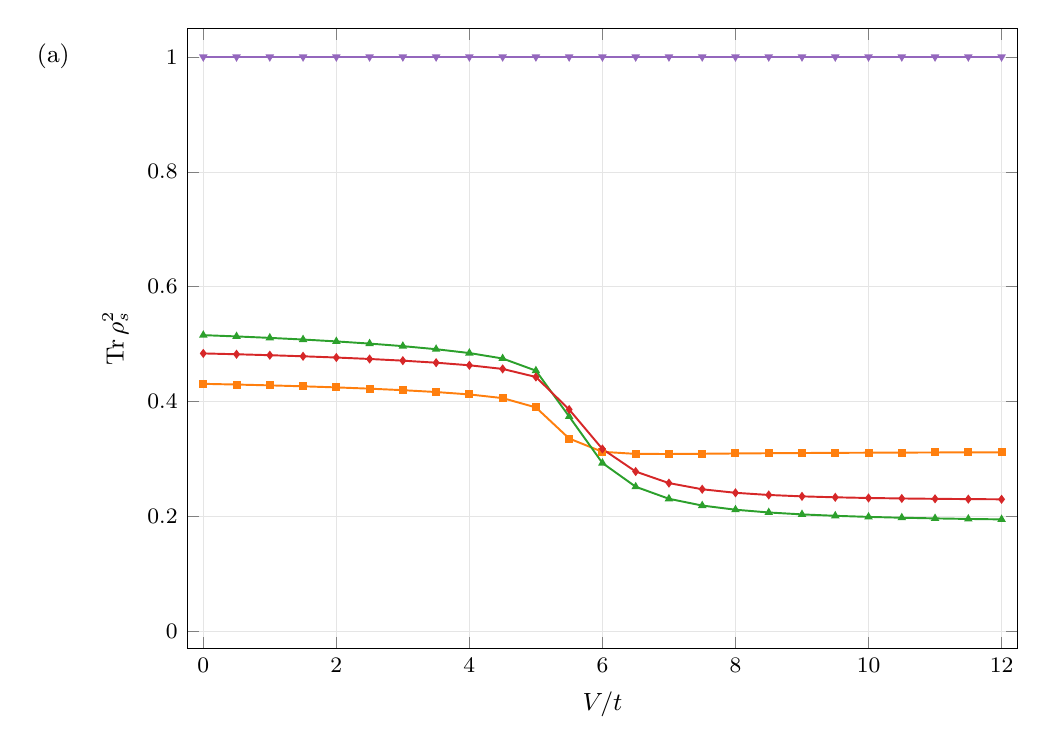
\begin{tikzpicture}
  \begin{axis}[
    width=\columnwidth,
    height=0.78\columnwidth,
    xlabel={$V/t$},
    ylabel={$\mathrm{Tr}\,\rho_s^2$},
    grid=both,
    grid style={line width=.1pt, draw=gray!20},
    tick label style={font=\footnotesize\rmfamily, /pgf/number format/fixed},
    label style={font=\small\rmfamily},
    scaled ticks=false,
    legend style={font=\scriptsize\rmfamily, draw=gray!40, at={(0.5,1.03)}, anchor=south, /tikz/every even column/.append style={column sep=6pt}},
    legend cell align={left},
    legend columns=2,
    ymin=-0.03,
    ymax=1.05,
    xmin=-0.24,
    xmax=12.24,
    after end axis/.append code={\node[anchor=east, font=\small\rmfamily] at (axis description cs:-0.13,0.954) {(a)};},
  ]
    \addplot[color=gmeC1, mark=square*, mark size=1.1pt, line width=0.7pt] coordinates {
        (0,0.430737) (0.5,0.429478) (1,0.428048) (1.5,0.42641)
        (2,0.42452) (2.5,0.42231) (3,0.419681) (3.5,0.416455)
        (4,0.412254) (4.5,0.405876) (5,0.389637) (5.5,0.335464)
        (6,0.312322) (6.5,0.308725) (7,0.308529) (7.5,0.308953)
        (8,0.309444) (8.5,0.309882) (9,0.310249) (9.5,0.310551)
        (10,0.310801) (10.5,0.311007) (11,0.31118) (11.5,0.311324)
        (12,0.311447)
    };
    \addplot[color=gmeC2, mark=triangle*, mark size=1.1pt, line width=0.7pt] coordinates {
        (0,0.515511) (0.5,0.513275) (1,0.510748) (1.5,0.507877)
        (2,0.50459) (2.5,0.500795) (3,0.496351) (3.5,0.491024)
        (4,0.484333) (4.5,0.474824) (5,0.453633) (5.5,0.373857)
        (6,0.29283) (6.5,0.25151) (7,0.230518) (7.5,0.218744)
        (8,0.2115) (8.5,0.206705) (9,0.203345) (9.5,0.200884)
        (10,0.199015) (10.5,0.197555) (11,0.196386) (11.5,0.195433)
        (12,0.194641)
    };
    \addplot[color=gmeC3, mark=diamond*, mark size=1.1pt, line width=0.7pt] coordinates {
        (0,0.483685) (0.5,0.482229) (1,0.480577) (1.5,0.478694)
        (2,0.47653) (2.5,0.474019) (3,0.471067) (3.5,0.467513)
        (4,0.463036) (4.5,0.456683) (5,0.442659) (5.5,0.385988)
        (6,0.317244) (6.5,0.277951) (7,0.257853) (7.5,0.247112)
        (8,0.240957) (8.5,0.23719) (9,0.234754) (9.5,0.233104)
        (10,0.231943) (10.5,0.2311) (11,0.23047) (11.5,0.229989)
        (12,0.229614)
    };
    \addplot[color=gmeC4, mark=triangle*, mark size=1.1pt, mark options={rotate=180}, line width=0.7pt] coordinates {
        (0,1) (0.5,1) (1,1) (1.5,1)
        (2,1) (2.5,1) (3,1) (3.5,1)
        (4,1) (4.5,1) (5,1) (5.5,1)
        (6,1) (6.5,1) (7,1) (7.5,1)
        (8,1) (8.5,1) (9,1) (9.5,1)
        (10,1) (10.5,1) (11,1) (11.5,1)
        (12,1)
    };
  \end{axis}
\end{tikzpicture}
